\section{Bragg-Reflexion}\label{sec:bragg}
Ziel ist es, mit einer Röntgenröhre Röntgenstrahlung zu erzeugen und das entstandene
Spektrum mithilfe der Bragg-Reflexion messen zu können. Fällt auf einen Kristall ein
paralleles Lichtbündel, so entsteht am Glanzwinkel $\vartheta$ konstruktive Interferenz.
Aus \cref{fig:bragg} lässt sich die Bragg-Bedingung für konstruktive Interferenz
herleiten. Diese lautet
\begin{equation}
	n\lambda = 2d\sin\vartheta
	\label{eq:bragg}
\end{equation}
mit der Beugungsordnung $n$, der Wellenlänge $\lambda$ und dem Gitterabstand $d$ \cite{wiki:bragg}.

\subsection{Aufbau}
Zur Erzeugung des Röntgenlichts wird ein Vollschutzröntgengerät verwendet, welches
freie Elektronen auf eine Anode beschleunigt und dadurch zu einem Teil ein kontinuierliches
Spektrum durch Bremsstrahlung entsteht und zum anderen Teil materialspezifische Linien
durch den photoelektrischen Effekt \cite{wiki:roentgenroehre}. Diese Linien werden
als charakteristische Röntgenstrahlung bezeichnet.\par
Mit einem Kollimator von \SI{1}{\mm} Spaltbreite wird ein paralleles Strahlenbündel erzeugt
und auf einen NaCl-Kristall gerichtet. Dieser ist in einem \SI{5}{\cm} Abstand zum
Kollimator auf der Halterung eines Goniometers befestigt, deren Neigunsgwinkel relativ zur Strahlung
eingestellt werden kann (siehe \cref{fig:aufbau-bragg}). Der Neigungswinkel entspricht dem Glanzwinkel $\vartheta$ aus
\cref{fig:bragg}.
Für einen Natrium-Chlorid-Kristall ist der doppelte Gitterabstand gegeben mit $2d = \SI{564.02}{\pm}$ \cite{ld_bragg}.
Um die Strahlung zu messen, wird am Goniometer ein Geiger-Müller-Zählrohr mit Kollimator befestigt mit einem
\SI{6}{\mm} Abstand zur Halterung und mit der Option
\verb|Coupled| am Experimentiergerät automatisch auf den entsprechenden Messwinkel gedreht.
Ein Geiger-Müller-Zählrohr ist ein gasgefüllter Kondensator, mit dem Teilchen durch Ionisation des Gases gemessen
werden können. In dem hier genutzten Betrieb kann durch eine vom Teilchen unabhängige Verstärkung lediglich
die Anzahl der Teilchen gemessen werden \cite{wermes}, was für diesen Versuch ideal ist, da die Energie
der Photonen nach \cref{eq:bragg} auf den Glanzwinkel abgebildet wird.\par

Der Goniometer-Aufbau ist in \cref{fig:aufbau-bragg} gezeigt.

\begin{figure}[htb]
	\centering
	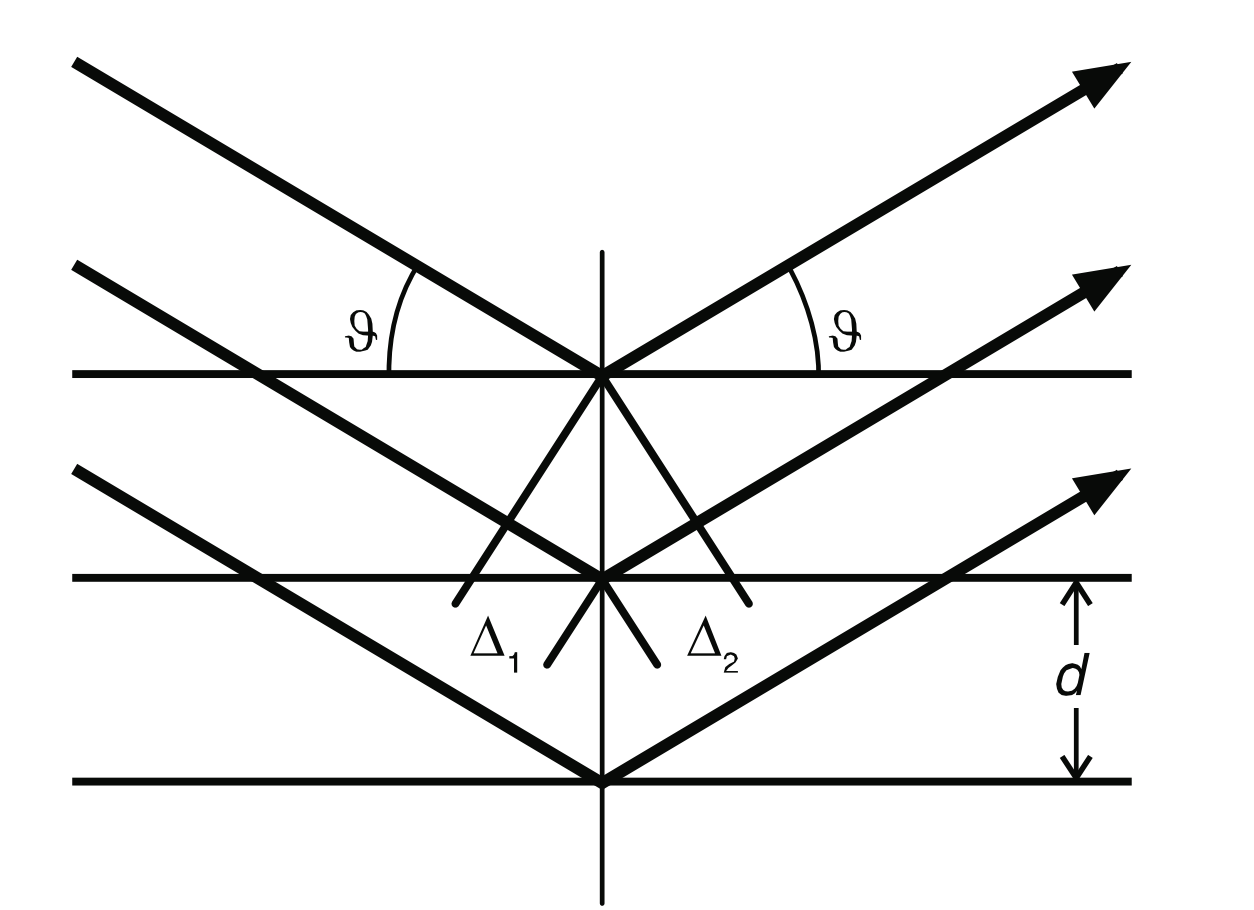
\includegraphics[width=0.6\linewidth]{bragg.png}
	\caption{Veranschaulichung der Bragg-Reflexion. Dargestellt sind zwei parallele Strahlen,
		die aufgrund der Wegdifferenz nach der Reflexion miteinander interferieren.}
	\label{fig:bragg}
\end{figure}

\newcommand\ebf[1]{\textbf{(#1)}}
\begin{figure}[htb]
	\centering
	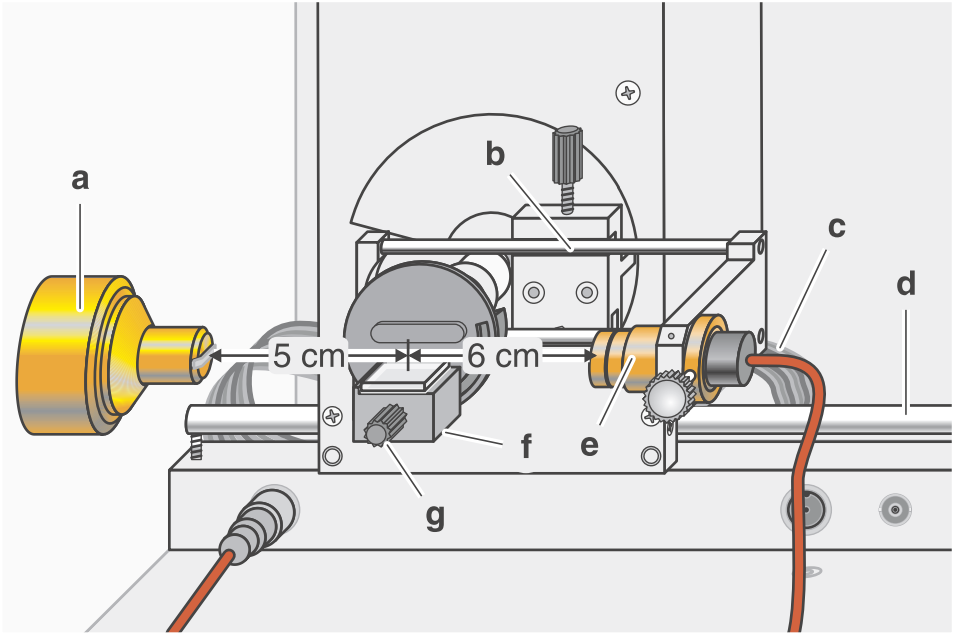
\includegraphics[width=0.6\linewidth]{aufbau-bragg.png}
	\caption{Aufbau auf dem Goniometer zur Messung des Röntgenspektrums mit einem NaCl-Kristall. \ebf a ist 
	Der Kollimator, \ebf b die Halterung des Zählrohrs, \ebf c das Kabel zur Verbindung des Zählrohrs mit 
	dem Computer und \ebf e der Kollimator davor. \ebf d ist die Stange, auf der das Goniometer verschoben
	werden kann, \ebf f die Halterung des Einkristalls und \ebf g die Schraube, mit der die Halterung 
	festgeschraubt werden kann.}
	\label{fig:aufbau-bragg}
\end{figure}

\subsection{Untersuchung einer unbekannten Anode}\label{sec:unbekannte_anode}
\subsubsection{Messung}
In das Messgerät wird eine Röntgenröhre mit unbekannter Anode eingesetzt und mit dem oben beschriebenen Aufbau
das dabei entstehende Röntgenspektrum gemessen. Hierfür wird eine Röhrenhochspannung von \SI{35.0}{\kilo\volt} und
ein Emissionsstrom von \SI{1}{\milli\ampere} eingestellt. Die Messzeit eines Winkelschritts liegt bei
$\Delta t = \SI{10}{\second}$
bei einer Winkelschrittweite von $\SI{0.1}{\degree}$. Der Messbereich wird auf \qtyrange{2.}{25.}{\degree} gestellt.
Somit wird in diesem Bereich vom Zählrohr die Anzahl der auftreffenden Photonen gemessen
und über das Zeitintervall geteilt, wodurch von dem genutzten Computer-Programm
\enquote{Röntgengerät} die mittlere Zählrate am dazugehörigen Winkel gespeichert wird. Alle
aufgenommenen Messwerte stehen in dem Sciebo-Ordner \textbf{HIER SCIEBO ORDNER}
zur Verfügung.

\subsubsection{Auswertung}
Das gemessene Spektrum ist in \cref{fig:anode-unbekannt-messung} zu beobachten. Erkennbar ist hierbei
ein kontinuierliches Spektrum mit Maximum bei etwa \qtyrange{4}{5}{\degree} und einen Abfall gegen 0
für hohe Winkel. Zusätzlich sei angemerkt, dass bei einer Spannung von \SI{35.0}{\kilo\volt}
Licht mit einer minimalen Wellenlänge von \SI{35.4}{\pm} erzeugt werden kann, was einem Glanzwinkel
von \SI{3.6}{\degree} entspricht. Dies kann mit der Messung bestätigt werden, jedoch ist ein geringer
Anstieg schon bei etwa \SI{3}{\degree} zu erkennen, wenn ein Hintergrundrauschen von ca. \SI{5}{\per\second}
angenommen wird. Dass die maximale Energie des Lichts höher ist als erwartet, wird ausgeschlossen. 
Die wahrscheinlichste Fehlerquelle hierfür sind Unsicherheiten durch den Aufbau. 
Das Strahlenbündel ist mit einer gewissen Unsicherheit nicht vollständig kollimiert und ist 
dadurch entweder leicht divergent oder konvergent, wodurch Licht einer Wellenlänge sich auf benachbarte
Winkel verteilt. Der Aufbau bestimmt somit auch maßgeblich die Breite der charakteristischen Linien, 
die in der Messung herausstechen.\par 
Als Winkelunsicherheit wird $\Delta\beta = \SI{0.01}{\degree}$ gewählt, da das Goniometer zweimal hintereinander 
kalibriert worden ist und dies die Unsicherheit dieser Kalibration darstellt. Da es sich hierbei um 
einen diskreten Messvorgang von unabhängigen Zählvorgängen handelt, sind die gemessenen Photonenzahlen 
Poisson-verteilt und besitzen die Unsicherheit $\Delta N = \sqrt{N}$. Für die mittlere Rate $n = N/t$ ergibt sich damit 
eine Unsicherheit von 
\begin{equation}
	\Delta n = \sqrt{\frac{n}{t}}.
	\label{eq:poisson_error}
\end{equation}\\\par
Die gemessenen Linien können mit einer Gauß-Funktion beschrieben werden:
\begin{equation}
	f(x,x_0,\sigma) = \frac{1}{\sqrt{2\pi}\sigma}\exp\qty(-\frac{(x-x_0)^2}{2\sigma^2}).
	\label{eq:gauss}
\end{equation}
Es muss jedoch beachtet werden, dass zum einen durch das kontinuierliche Spektrum und dem Rauschen 
ein zusätzlicher Offset mit berücksichtigt werden muss. Dieser Offset kann in einem Bereich um 
die Gauß-Kurve linear angenähert werden mit $g(x) = mx + n$. Einige Linien hier und in weiteren Messungen sind so nah beieinander, 
dass mehrere Gauß-Kurven als Summe betrachtet werden müssen. Im Allgemeinen lässt sich also in einem 
gewählten Intervall eine Funktion der Form 
\begin{equation*}
	f(x) = \sum_{k=1}^N A_kf(x,x_{0,k}, \sigma_k) + g(x)
\end{equation*}
finden, die den Verlauf der mittleren Zählrate angemessen beschreiben kann. Die Regression wurde hier und im weiteren 
Verlauf mit dem Python 
Modul \verb|odr| des Pakets \verb|scipy| auf sinnvoll 
gewählten Intervallen durchgeführt. Dabei wird die Güte der Anpassungen mit dem $\chi^2$ beurteilt, 
wobei mit $\chi^2$ im Folgenden eigentlich das Chi-Quadrat geteilt durch die Freiheitsgrade gemeint ist 
\cite{wiki:reduced_chi_square}. Wie in der Legende von \cref{fig:anode-unbekannt-messung} zu sehen, befindet 
sich das Chi-Quadrat für alle sechs Regressionen im Bereich von \num{0.83} bis \num{5.53} und modellieren 
damit die Messwerte sehr gut.\par

\begin{figure}[htb]
	\centering
	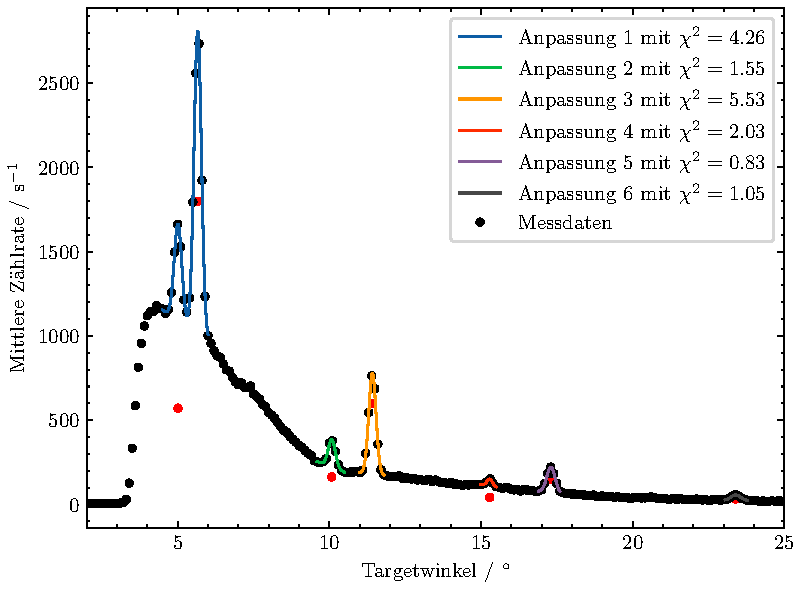
\includegraphics[width=0.6\linewidth]{anode-unbekannt.pdf}
	\caption{Messung des Röntgenspektrums einer unbekannten Anode. Die hier eingezeichneten Fehler sind zu klein, um
	sichtbar zu sein.}
	\label{fig:anode-unbekannt-messung}
\end{figure}

Aus den Modellierungen lassen sich die Winkel $\vartheta$ der charakteristischen Linien ablesen und daraus mit 
\cref{eq:bragg} die Größe $n\lambda$. Mit Gaußscher Fehlerfortpflanzung \cite{wiki:fehlerfortpflanzung}
ist die dazugehörige Unsicherheit mit 
\begin{equation}
	\Delta(n\lambda) = 2d\cos\vartheta\Delta\vartheta
	\label{eq:bragg_uncertainty}
\end{equation}
gegeben. Da Energie und Wellenlänge eines Photons eindeutig miteinander verknüpft sind lässt sich daraus 
die Energie pro Beugungsordnung bestimmen mit
\begin{equation}
	\frac{E}{n} = \frac{hc}{\lambda}, \qquad \Delta\qty(\frac{E}{n}) = \frac{E}{n}\frac{\Delta\lambda}{\lambda}.
	\label{eq:energy_photon}
\end{equation}

Bekannterweise sind hier $h=\SI{6.62606896e-34}{\joule\second}$ und $c=\SI{299 792 458}{\meter\per\second}$ 
\cite{Demtröder:829119}.

\begin{table}[htbp]
   \centering
\caption{Bestimmung der Wellenlängen und Energien pro Beugungsordnung aus dem gemessenen Spektrum der unbekannten Anode}
\begin{tabular}{c c c}
\hline Winkel $\vartheta/ \unit{\degree}$ & Wellenlänge $n\lambda / \unit{\pm}$ & Energie $En^{-1} / \unit{\kilo\electronvolt}$  \\ 
\hline
$\num{5.011\pm 0.006}$ & $\num{49.26\pm 0.06}$ & $\num{25.17\pm 0.03}$ \\
$\num{5.661\pm 0.005}$ & $\num{55.63\pm 0.05}$ & $\num{22.287\pm 0.019}$ \\
$\num{10.082\pm 0.007}$ & $\num{98.73\pm 0.06}$ & $\num{12.558\pm 0.008}$ \\
$\num{11.420\pm 0.004}$ & $\num{111.67\pm 0.04}$ & $\num{11.102\pm 0.004}$ \\
$\num{15.292\pm 0.019}$ & $\num{148.75\pm 0.18}$ & $\num{8.34\pm 0.01}$ \\
$\num{17.307\pm 0.005}$ & $\num{167.78\pm 0.04}$ & $\num{7.3895\pm 0.0017}$ \\
$\num{23.402\pm 0.014}$ & $\num{224.01\pm 0.13}$ & $\num{5.535\pm 0.004}$ \\
\hline\end{tabular}
\label{tab:anode-unbekannt}
\end{table}

An den Wellenlängen in \cref{tab:anode-unbekannt} ist zur erkennen, dass die dritte bis einschließlich 
sechste Wellenlänge jeweils im $2\sigma$-Bereich Vielfache von den ersten beiden Wellenlänge $\SI{49.26\pm 0.06}{\pm}$
und $\SI{55.63\pm 0.05}{\pm}$ in der zweiten Ordnung; die dritte Ordnung weist eine leichte Diskrepanz von 
unter \SI{1}{\percent} auf. In der vierten Ordnung ist nur noch die zweite Linie erkennbar. Da bis zur vierten 
Ordnung Vielfache eines Wellenlängenpaares gefunden werden konnten, kann mit großer Sicherheit 
behauptet werden, dass die ersten beiden Wellenlängen zwei Linien des charakteristischen Spektrums 
der Anode darstellen und alle Weiteren die gleichen Linien höher Beugungsordnungen sind.\par
Es deutet darauf hin, dass die Anode hierbei aus Silber besteht, welches 
vier Linien K$_\mathrm{\beta_{4/5}} = \SI{49.3}{\pm}$,  K$_\mathrm{\alpha_3}=\SI{55.9}{\pm}$
und K$_\mathrm{\alpha_2}=\SI{56.3}{\pm}$ besitzt \cite{nist_xray_database}, die zur Feinstrukturaufspaltung gehören und 
deshalb nicht einzeln aufgelöst werden können (die K$_\beta$-Linien gehören zur 
Hyperfeinstruktur, da auf die erste Nachkommastelle gerundet noch keine 
Aufspaltung erkennbar ist). Die K$_\beta$-Linie liegt im $1\sigma$-Bereich 
der Messung und beide K$_\alpha$-Linien liegen nahezu gleich verteilt um den Messwert herum, weshalb 
höchstwahrscheinlich die Messung den Mittelwert beider Linien gemessen hat.

\subsection{Feinstrukturaufspaltung der K$_\alpha$-Linie von Molybdän}
Aufgrund der Spin-Bahn-Kopplung zwischen Spin und Bahndrehimpuls eines an einen Atomkern 
gebundenen Elektrons ist die Bindungsenergie von Bahndrehimpuls und Gesamtdrehimpuls abhängig, was 
zu einer Aufspaltung der von den Hauptquantenzahl bestimmten Grobstruktur in die Feinstruktur führt
\cite{Demtröder:829119}. Da die Energiedifferenz dieser Linien jedoch gering ist, sind hohe 
Auflösungen bei der Messung nötig. Hierfür muss der Aufbau nicht verändert werden, sondern lediglich 
der Messvorgang. Da nach \cref{eq:bragg_uncertainty} bei höherer Ordnung $n$ die Winkeldifferenz zwischen 
zwei Linien höher sein muss, wird für die Untersuchung der Feinstruktur die vierte Beugungsordnung gemessen.

\subsubsection{Messung}
Es wird in das Messgerät eine Röntgenröhre mit einer Molybdän-Anode eingesetzt. Hier wird 
erneut eine Röhrenhochspannung von \SI{35.0}{\kilo\volt} und
ein Emissionsstrom von \SI{1}{\milli\ampere} eingestellt. Die Messzeit eines Winkelschritts liegt diesmal
bei $\Delta t = \SI{120}{\second}$ um präzisere Messergebnisse zu bekommen.
Bei einer Winkelschrittweite von $\SI{0.01}{\degree}$ wird der Messbereich auf \qtyrange{28.5}{32.0}{\degree} gestellt.

\subsubsection{Auswertung}

Die Fehler wurden gleich wie in \cref{sec:unbekannte_anode} gesetzt. In \cref{fig:feinstruktur} ist die 
Messung der Feinstruktur mit dazugehöriger Anpassung an die Gaußkurven zu sehen. Visuell stimmt die Regressionskurve 
mit den Messungen überein, was von einem $\chi^2 = 1.96$ bestätigt wird. Auch hier konnten wieder mit 
\cref{eq:bragg} und \cref{eq:energy_photon} die Wellenlängen und Energien der Linien berechnet werden. 
Die berechneten Messwerte sind \cref{tab:feinstruktur} zu entnehmen. Wie zu sehen ist, sind die Messwerte 
auf drei signifikante Stellen identisch, da jedoch die resultierenden Fehler gering sind, liegen die 
theoretischen Referenzwerte nicht im $3\sigma$-Bereich der Messung. Möglicherweise sind die mit \SI{0.01}{\degree}
abgeschätzten Fehler zu klein gewählt.\par 
Das Dublett der Wellenlängen $\lambda_1$ und $\lambda_2$ besitzt einen Abstand von 
\begin{equation*}
	\Delta\lambda = \lambda_1 - \lambda_2,\qquad \Delta(\Delta\lambda) = 
	\sqrt{(\Delta\lambda_1)^2+ (\Delta\lambda)^2},
\end{equation*}
was hier einen Abstand von 
\begin{equation}
	\Delta\lambda_\mathrm{Exp} = \SI{0.444\pm 0.008}{\pm},\qquad
	\Delta\lambda_\mathrm{Ref} = \SI{0.428\pm0.004}{\pm}
\end{equation}
ergibt und somit der Literaturwert auch hier nicht im $3\sigma$-Bereich der Messung liegt. Damit kann eine 
systematische Unsicherheit ausgeschlossen werden, weshalb die hier vorhandene Abweichung 
aus einer nicht berücksichtigten statistischen Unsicherheit entspringen muss. Die Lage des Kristalls 
kann hierbei die Messung verfälschen. Sind die bestrahlen Ebenen des NaCl-Kristalls nicht 
genau parallel zum Tisch, so verfälscht dies die Winkelmessung.

\begin{figure}[htb]
	\centering
	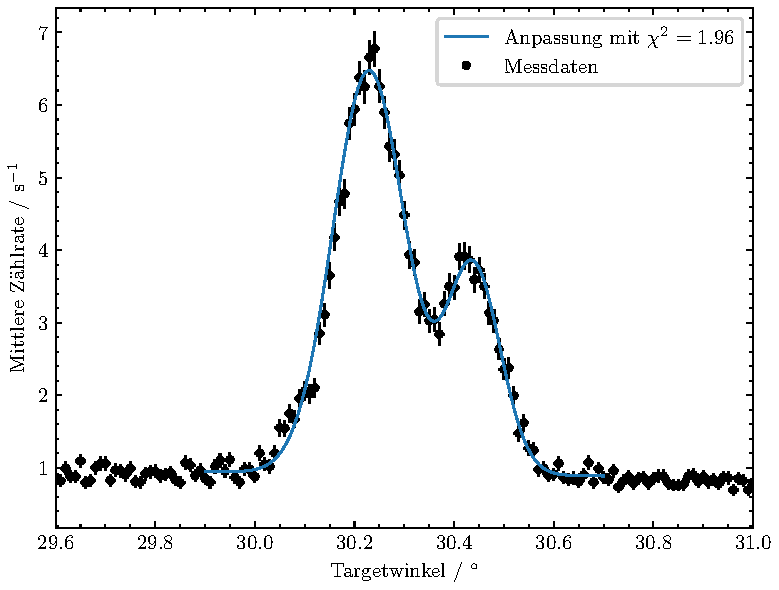
\includegraphics[width=0.6\linewidth]{feinstruktur.pdf}
	\caption{Messung der Feinstruktur der K$_\alpha$-Linie von Molybdän in 4. Beugungsordnung.}
	\label{fig:feinstruktur}
\end{figure}

\begin{table}[htbp]
   \centering
\caption{Bestimmung der Wellenlängen und Energien aus der Messung der Feinstrukturaufspaltung}
\begin{tabular}{c c c}
\hline Winkel $\theta/ \unit{\degree}$ & Wellenlänge $\lambda / \unit{\pm}$ & Energie $E / \unit{\kilo\electronvolt}$  \\ 
\hline
$\num{30.229\pm 0.003}$ & $\num{70.987\pm 0.005}$ & $\num{17.4657\pm 0.0012}$ \\
$\num{30.438\pm 0.003}$ & $\num{71.431\pm 0.006}$ & $\num{17.3571\pm 0.0015}$ \\
\hline\end{tabular}
\label{tab:feinstruktur}
\end{table}